% !TEX encoding = UTF-8 Unicode
\documentclass[12pt,twoside,a4paper]{report}
\setcounter{tocdepth}{2}
\usepackage[]{geometry}
\setlength{\headheight}{15.0pt}
\usepackage[utf8]{inputenc}
\usepackage[T1]{fontenc}
\usepackage[francais]{babel}
\usepackage{graphicx}

% header
\usepackage{fancyhdr}
\pagestyle{fancy}

% code listings
\usepackage{listings}

\usepackage[usenames,dvipsnames,svgnames,table,xcdraw]{xcolor}
\usepackage{pdfpages}

\definecolor{olivegreen}{HTML}{3C8031}

\usepackage[T1]{fontenc}
\usepackage[scaled]{beramono}
\newcommand\Small{\fontsize{9}{9.2}\selectfont}
\newcommand*\LSTfont{\Small\ttfamily\SetTracking{encoding=*}{-60}\lsstyle}

\definecolor{lightgray}{rgb}{.9,.9,.9}
\definecolor{darkgray}{rgb}{.4,.4,.4}
\definecolor{purple}{rgb}{0.65, 0.12, 0.82}
\lstdefinelanguage{JavaScript}{
  keywords={break, case, catch, continue, debugger, default, delete, do, else, false, finally, for, function, if, in, instanceof, new, null, return, switch, this, throw, true, try, typeof, var, void, while, with},
  morecomment=[l]{//},
  morecomment=[s]{/*}{*/},
  morestring=[b]',
  morestring=[b]",
  ndkeywords={class, export, boolean, throw, implements, import, this},
  keywordstyle=\color{blue}\bfseries,
  ndkeywordstyle=\color{darkgray}\bfseries,
  identifierstyle=\color{black},
  commentstyle=\color{purple}\ttfamily,
  stringstyle=\color{red}\ttfamily,
  sensitive=true
}

\lstset{ %
  basicstyle=\footnotesize\ttfamily,        % the size of the fonts that are used for the code
  breakatwhitespace=false,         % sets if automatic breaks should only happen at whitespace
  breaklines=true,                 % sets automatic line breaking
  commentstyle=\color{olivegreen},    % comment style
  escapeinside={\%*}{*)},          % if you want to add LaTeX within your code
  extendedchars=true,              % lets you use non-ASCII characters; for 8-bits encodings only, does not work with UTF-8
  frame=single,	                   % adds a frame around the code
  keepspaces=true,                 % keeps spaces in text, useful for keeping indentation of code (possibly needs columns=flexible)
  keywordstyle=\color{blue},       % keyword style
  lineskip={-1.5pt},
  numbers=left,                    % where to put the line-numbers; possible values are (none, left, right)
  numbersep=5pt,                   % how far the line-numbers are from the code
  numberstyle=\tiny\color{black}, % the style that is used for the line-numbers
  rulecolor=\color{black},         % if not set, the frame-color may be changed on line-breaks within not-black text (e.g. comments (green here))
  showspaces=false,                % show spaces everywhere adding particular underscores; it overrides 'showstringspaces'
  showstringspaces=false,          % underline spaces within strings only
  showtabs=false,                  % show tabs within strings adding particular underscores
  stepnumber=1,                    % the step between two line-numbers. If it's 1, each line will be numbered
  stringstyle=\color{purple},     % string literal style
  tabsize=2,	                   % sets default tabsize to 2 spaces
}

% link
\usepackage{hyperref}

% glossary
\usepackage[automake]{glossaries}

\usepackage{bytefield}

\usepackage{amsmath}

\usepackage{subfig}

\usepackage{caption}

\usepackage[section]{placeins}

\usepackage[export]{adjustbox}

\usepackage{wrapfig}

\usepackage{rotating}

\usepackage{longtable}

\newcommand\MyLBrace[2]{%
  \left.\rule{0pt}{#1}\right\}\text{#2}}

\newcommand\MyRBrace[2]{%
  \left.\rule{0pt}{#1}\text{#2}\right\{}


\makeglossaries

\newglossaryentry{mot}
{
	name=mot,
	description={est fun.}
}


\begin{document}

\includepdf[pages={1}]{images/garde.pdf}

\def\myTitle{Développement d'une Application Web pour la Visualisation et la Recherche de Données Médicales}
\def\myName{Kewin Dousse}
\def\myUni{HES-SO}
\def\myDepartment{TIC}
\def\mySupervisors{Sandy Ingram}
\def\myExpert{?}


\begin{abstract}

Le but de ce projet est de concevoir et d'implémenter un outil d'analyse de comportement d'utilisateurs d'applications Web pour révéler les potentiels de détection de profile des personnes (préférences, centre d'intérêt, orientations et opinions) en analysant les interactions et les informations échangées avec les applications Web.

\smallskip
\noindent \textbf{Keywords.} Web, Big Data, Privacy, Profiling

\end{abstract}
\setcounter{page}{3}
\hypersetup{pageanchor=true}

\tableofcontents
\listoffigures

\chapter{Introduction}
\section{Contexte}

	L'hôpital orthopédique du \gls{CHUV} utilise actuellement un fichier Excel partagé pour conserver les données médicales des patients. Bien que fonctionnelle, cette méthode est fastidieuse à la fois pour l'entrée de nouvelles données que pour la recherche parmi celles-ci, et ne possède pas de réel point positif autre que la facilité initiale de la mise en place.

	Le but de ce projet est de concevoir et développer une application Web multiplateforme pour la recherche et la visualisation de ces données médicales. Le projet comporte deux challenges techniques centraux :
	\begin{enumerate}
		\item L’architecture désirée nécessitera donc un développement sur toutes les couches du système, autrement dit « full stack ».
		\item L’aspect multiplateforme nécessitera l’utilisation d’outils et de librairies récentes.
	\end{enumerate}
	Ce projet est mené dans un but double : Il aura à la fois une utilité scientifique en tant que base de données pour des futures études, et une utilité clinique par l’utilisation de son interface par le personnel.

\section{Objectifs}

	À la fin du projet, nous serons en possession d’une application web multiplateforme permettant de :
	\begin{itemize}
		\item Rechercher et visualiser des données médicales
		\item Rechercher, visualiser et modifier des données de patients
		\item Insérer des données médicales
	\end{itemize}

	Un objectif est qualifié de secondaire, et sera réalisé en fonction de l’avancement du projet :
	\begin{itemize}
		\item Produire et montrer des statistiques sur les patients et les cas
	\end{itemize}

\section{Contraintes}

	Le développement du projet va se faire autour de quelques contraintes définies :
	\begin{itemize}
		\item L’application doit converser avec une base de données MySQL déjà existante.
		\item L’application doit être adaptée à une utilisation à la fois sur un appareil desktop, et sur un appareil mobile, ainsi que convenir à la plupart des navigateurs récents.
	\end{itemize}

\section{Méthodologie}

	Le développement se fera de manière itérative, afin de produire plusieurs maquettes et prototypes, avec des degrés de fidélité augmentant au fil du projet. 
	Le but est d'utiliser une méthodologie agile afin de pouvoir rapidement proposer des
	prototypes, et avoir des retours de clients assez tôt. On désire s'assurer que l'on produit une solution adaptée aux besoins du client.
\chapter{Analyse}
%%%%%%%%%%%%%%%%%%%%%%%%%
%                          %
% ----- INTRODUCTION ----- %
%                          %
%%%%%%%%%%%%%%%%%%%%%%%%%%

\section{Analyse des besoins}

	\subsection{Enquête}

	Afin de comprendre correctement les demandes des clients, il a été nécessaire de mener une enquête sur le public cible en procédant à une interview de quelques personnes concernées parmi le public cible. Une rencontre a donc eu lieu avec Mme. Sandy Ingram, M. Alain Farron, M. Alexandre Terrier et M. Fabio Becce. Cette réunion a donné lieu à plusieurs questions et des réponses de la part de toutes les personnes, qui ont aidé à définir quels étaient les besoins du public ciblé.

	La solution sera donc utilisée par deux catégories de personnes qui vont vouloir
	en tirer des informations différentes :

	\begin{itemize}
		\item Des médecins vont vouloir utiliser l'application pour visualiser
		et modifier les données des patients directement.
		\item Des scientifiques vont vouloir, dans un deuxième temps,
		extraire des informations statistiques sur les données elles-mêmes,
		afin de pouvoir par exemple mener des études approfondies sur les nombres.
	\end{itemize}

	En plus des informations du public cible, nous avons appris plusieurs informations essentielles sur le fonctionnement demandé de plusieurs des pages :

	\begin{itemize}
		\item Un cas peut avoir plusieurs CT scans associés à lui.
		\item Pour un patient, on aimerait voir la liste de ses cas, et rapidement voir son cas "primaire" (le plus récent).
		\item Pour un patient, on aimerait voir principalement son diagnostique, et son traitement.
		\item Pour un cas, on aimerait voir touts les scans, ainsi que toutes les mesures de ces scans.
	\end{itemize}

	Ces critères ont été pris en compte pour la suite du développement de l'application. Certains points sont restés flous, mais non bloquants pour l'avancement de l'application ; est-ce que l'application doit permettre l'ajout de mesures ? Est-ce que l'application doit permettre l'ajout de patients ? Mais ces mêmes questions ont été éclaircies à l'avenir par des échanges de mails, et également une réunion par Skype.

	En conclusion de cette réunion, nous pouvons tout de même regrouper les besoins du client en deux catégories.

	\subsection{Besoins cliniques}

		Des médecins et du personnel soignant vont être encouragés à utiliser l'application, et ceux-ci veulent pouvoir accéder à une vue par patient, ce qui est le plus naturel pour eux. Leur but sera d'obtenir, de visualiser et de modifier des données reliées à un patient. Il sera plus important de pouvoir accéder aux données complètes d'une personne en particulier, ainsi que tous les cas associés à cette personne. En effet, une personne peut être enregistrée dans la base de données pour plusieurs raisons : Un "cas" correspond à une anomalie à traiter. Une personne peut par exemple en accumuler plusieurs sur le temps. Il sera dans ce cas probablement intéressant de regarder l'évolution d'une personne sur le temps, regroupant tous les cas liés.

		Cette catégorie de personne veut pouvoir afficher ou cacher certaines catégories d'informations. Par exemple, il arrivera qu'un médecin veuille consulter rapidement une fois les données des scans du patient, et une autre fois les données concernant son traitement. La solution est donc de ne pas tout afficher directement, mais de laisser à l'utilisateur la possibilité de filtrer les résultats. Certaines informations seront affichées par défaut car très souvent consultées, comme par exemple le traitement actuel du patient ou son diagnostic. Mais d'autres catégories d'informations telles que les mesures des scans ne seront pas visible d'office et pourront être activées lors de la recherche.

	\subsection{Besoins scientifiques}
	
		L'application va cibler une catégorie d'utilisateurs qui est intéressé à obtenir des informations brutes sur les données de la base elle-même afin de les intégrer par exemple au sein d'études scientifiques, et dans un deuxième temps de produire des statistiques. Pour eux, les données spécifiques à un patient sont moins importantes, mais il est capital de pouvoir naviguer parmi les informations de la manière la plus structurée possible. Le but sera de regrouper les informations par cas, et non pas par personne. Il a été défini selon les besoins que plusieurs scans peuvent être liés à un seul cas.

		Cette catégorie de personne va vouloir accéder aux données "brutes" plus rapidement : Mesures des scans, images des scans par exemple. Comme pour la vue des patients, la vue des cas affichera certaines qu'une partie des informations par défaut pour des raisons de lisibilité. Ici à nouveau, il sera possible d'activer ou de désactiver l'affichage d'autres catégories d'informations qui sont ici moins importantes, comme par exemple le diagnostic du patient.

\section{Analyse technologique}

	Le projet comprend un challenge technologique : Le but est d'utiliser une ou plusieurs technologies de pointes dans le web. Mais bien qu'il s'agisse du challenge principal, plusieurs aspects surviennent lors de l'analyse des différentes couches de l'application.

	\subsection{Base de données}

		Le client possède actuellement les données des patients dans un fichier
		Excel. Afin de migrer ces données vers une base de données, celui-ci
		nous a envoyé un schéma montrant la structure qu'il a mise en place. La
		figure~\ref{schema_db} présente ce fichier qui, après une analyse,
		semble correspondre aux besoins qu'il demande ainsi qu'à la structure
		actuelle des données du fichier Excel.

		\begin{figure}[!h]
			\centering
			\includegraphics[width=1\textwidth]{images/analyse/SQLshoulderDatabase_reduced}
			\caption{Le schéma de la base de données reçu.}
			\label{schema_db}
		\end{figure}

		Nous allons donc prendre ce schéma comme référence pour la suite de l'analyse et du développement du projet.

	\subsection{Technologies}

		En plus de l'approche orientée utilisateur du projet, le but est également de découvrir et d'apprendre à utiliser certaines des plus récentes librairies du web. Pour ce projet, le choix logique a été fait de se concentrer une technologie servant à créer des interfaces utilisateur : React.

		Pour l'apprentissage de cette technologies et des librairies qui lui sont proches, j'ai suivi un tutoriel en plusieurs vidéo. Cette liste de vidéo est disponible sur YouTube\cite{learncode-academy}. 

		\subsubsection{React}\label{techno-react}
		
			\paragraph{Approche}

			Développée par Facebook le milieu de l'année 2013, React est "Une librairie JavaScript pour la création d'interfaces utilisateur"\cite{react}, traduit littéralement depuis le site officiel. React s'occupe donc strictement de la vue de l'application. Ce qui démarque principalement React des autres librairies similaires comme AngularJS est sa performance.

			La principale raison des performances élevées de React est dans le fait de conserver, en plus de la page affichée actuellement à l'écran (le DOM), un "DOM virtuel". Ce DOM virtuel est en pratique une copie en mémoire des éléments affichés à l'écran. La gestion habile de ce DOM virtuel permet à React de n'actualiser que les strictes parties de la page qui ont besoin de l'être, au moment où React le décide. Cela lui permet d'éviter beaucoup de rafraîchissements inutiles, que les autres librairies se devraient d'effectuer.

			\begin{figure}[h]
				\centering
				\includegraphics[width=0.8\textwidth]{images/analyse/virtualDOM}
				\caption{Le Virtual DOM est une étape intermédiaire entre React et le DOM\cite{valuecoders-choosereact}}
				\label{schema_virtualDOM}
			\end{figure}

			Le fait que le changement du DOM soit le principal élément lent dans presque tout code JavaScript permet donc à React de se démarquer.

			Une autres des caractéristiques de React est l'encouragement à écrire des composants réutilisables. De plus, bien que React ait été designé pour créer des interfaces web, il est aujourd'hui possible d'utiliser React ainsi que ses composants pour créer bien d'autres interfaces que du HTML. Par exemple, Facebook développe également depuis 2015 "React Native", qui permet d'utiliser des composants React pour créer des applications smartphone natives. Depuis, encore d'autres librairies ont constaté la puissance de React et tentent d'en tirer parti en dehors du navigateur.

			\paragraph{Tutoriel}

			Bien que React soit une librairie JavaScript, il est très recommandé de se construire un environnement de développement avec des outils adaptés afin de pouvoir développer correctement. Avec l'arrivée des gestionnaires de paquets tels que npm pour JavaScript, il serait une perte de temps de s'encombrer manuellement de toutes les étapes de recherche de dépendances de librairies, de leur assemblage, etc. Nous n'allons pas nous étendre sur tous les fichiers de configurations, mais allons lister les outils utiles pour React et allons expliquer la logique de fonctionnement principale de la librairie.

			\subparagraph{Node.js et npm}

			Nous allons partir du principe que la version 6.10.1 LTS de Node.js\cite{nodejs} (ainsi que npm\cite{npm}, qui est installé avec) sont installés sur la machine.

			Afin d'utiliser npm, nous allons créer un fichier de package, nommé 'package.json'. Ce fichier représente notre package d'application, et liste les librairies nécessaires pour le projet.

			\subparagraph{Dépendances}

			React lui-même est très puissant, mais il ne s'agit que du coeur logique du framework. D'autres librairies sont utilisées en cohésion avec React afin de par exemple générer du html. La figure~\ref{analyse_tutoriel_package}`montre' le contenu d'un fichier 'package.json' d'exemple, exposant des librairies quasi indispensables pour l'utilisation de React.

			\begin{figure}[!h]
				\begin{lstlisting}[]
{
  "name": "tutoriel",
  "version": "0.0.1",
  "description": "",
  "main": "webpack.config.js",
  "dependencies": {
    "react": "^15.4.2",
    "react-dom": "^15.4.2",
    "react-router": "^4.0.0",
    "react-router-dom": "^4.0.0-beta.8",
    "react-tap-event-plugin": "^2.0.1",
    "webpack": "^2.2.1",
    "webpack-dev-server": "^2.4.2"
  },
  "devDependencies": {},
  "scripts": {
    "dev": "webpack-dev-server --content-base src --inline --hot",
  },
  "author": "",
  "license": "ISC"
} \end{lstlisting}
				\caption{Fichier \texttt{package.json}}
				\label{analyse_tutoriel_package}
			\end{figure}

			On peut y voir les dépendances suivantes :

			\begin{itemize}
				\item \texttt{react} : Coeur logique de React.
				\item \texttt{react-dom} : Permet à React d'interagir avec le DOM.
				\item \texttt{react-router} : Permet à React d'interpréter des liens.
				\item \texttt{react-router-dom} : Fait le lien entre \texttt{react-router} et \texttt{react-dom}.
				\item \texttt{react-tap-event-plugin} : Corrige un bug pour que les interactions fonctionnent sur smartphone.
				\item \texttt{webpack} : Permet de "compiler" plusieurs scripts et librairies en un seul fichier JavaScript.
				\item \texttt{webpack-dev-server} : Permet de simplifier l'utilisation de \texttt{webpack} lors du développement.
			\end{itemize}

			\subparagraph{webpack et JSX}

			\texttt{webpack}\cite{webpack} est ici utile pour n'obtenir qu'un seul fichier JavaScript, très simple à utiliser avec une page HTML. Il est très recommandé de l'utiliser en cohésion avec React, mais son utilisation est optionnelle et sa configuration ne sera pas discutée ici. Les morceaux de code qui apparaîtront utiliseront tout de même la syntaxe JSX\cite{jsx}, qui est un sucre syntactique pour JavaScript. Il permet principalement d'écrire du code HTML dans du JavaScript. webpack, ainsi que d'autres technologies similaires, permettent de compiler cette syntaxe en JavaScript classique. Il est aussi tout à fait possible de ne pas utiliser JSX et d'écrire du JavaScript conventionnel simplement. La figure \ref{analyse_code_jsx} montre un code JSX, et la figure \ref{analyse_code_js} montre son équivalent JavaScript.

			\begin{figure}[!h]
				\begin{lstlisting}[language=html]
<MyButton color="blue" shadowSize={2}>
  Click Me
</MyButton> \end{lstlisting}
				\caption{Code JSX}
				\label{analyse_code_jsx}
			\end{figure}

			\begin{figure}[!h]
				\begin{lstlisting}[language=JavaScript]
React.createElement(
  MyButton,
  {color: 'blue', shadowSize: 2},
  'Click Me'
) \end{lstlisting}
				\caption{Equivalent compilé en JavaScript}
				\label{analyse_code_js}
			\end{figure}

			\subparagraph{Versions des librairies}

			Il est également à noter que React et d'autres librairies qu'il utilisent sont encore à ce jour énormément en développement, et il n'est pas rare de voir l'API changer, parfois excessivement souvent (j'ai pu voir des séries de changements conséquents à moins de 6 mois d'écart pour certaines librairies).

			Il est donc important de remarquer les versions utilisées des librairies, sur lesquelles se baseront à la fois le code du projet ainsi que ce guide d'utilisation. À noter également que les versions notées ici peuvent être utilisées ensemble, mais que cela n'est pas toujours le cas : Très souvent, une version d'une librairie va demander une version minimum d'une autre.

			\subparagraph{Composants}

			Le développement d'une application utilisant React repose sur la déclaration et l'utilisation de Composants. Un composant peut être vu comme un élément HTML possédant sa propre intelligence, indépendant des autres parties de la page. La figure \ref{analyse_composant_react} montre un exemple de code d'un composant simple.

			\begin{figure}[!h]
				\begin{lstlisting}[language=JavaScript]
class ShoppingList extends React.Component {
  render() {
    return (
      <div className="shopping-list">
        <h1>Shopping List for {this.props.name}</h1>
        <ul>
          <li>Instagram</li>
          <li>WhatsApp</li>
          <li>Oculus</li>
        </ul>
      </div>
    );
  }
}

// Example usage: <ShoppingList name="Mark" /> \end{lstlisting}
				\caption{Code d'un composant "\texttt{ShoppingList}", tiré de \cite{tutorial-react}}
				\label{analyse_composant_react}
			\end{figure}

			Voici les éléments qui constituent ici ce Composant :

			\begin{itemize}
				\item La méthode \texttt{render()} doit retourner une description de l'élément à afficher, soit ici un élément HTML (décrit avec la syntaxe JSX) en contenant plusieurs autres. Il s'agit là de la représentation qu'aura ce Composant lorsqu'il sera affiché dans la page HTML.
				\item Le paramètre \texttt{{this.props.name}}. Il s'agit là de code JavaScript : \texttt{this} se réfère à cette classe React, et \texttt{props} est un objet. \texttt{props} signifie 'propriétés', et c'est cet objet qui va généralement contenir les propriétés d'un élément React. Ici, une propriété est le nom \texttt{name}.
			\end{itemize}

			\subparagraph{Composition de Composants}

			Ici, le composant se constitue uniquement d'éléments HTML. Mais l'intérêt vient de la possibilité d'utiliser d'autres Composants à l'intérieur de la définition d'un de ces Composants. Par exemple, si nous avons décrit un Composant \texttt{Liste} dans notre code, nous pourrions l'utiliser ici à la place de l'élément HTML \texttt{ul} par exemple. Ainsi, la figure \ref{analyse_composant_react_2} montre cette modification apportée à notre décrit précédemment. 

			\begin{figure}[!h]
				\begin{lstlisting}[language=JavaScript]
class ShoppingList extends React.Component {
  render() {
    return (
      <div className="shopping-list">
        <h1>Shopping List for {this.props.name}</h1>
        <List values={['Instagram', 'WhatsApp', 'Oculus']}>
      </div>
    );
  }
}

// Example usage: <ShoppingList name="Mark" /> \end{lstlisting}
				\caption{Code modifié en utilisant un Composant}
				\label{analyse_composant_react_2}
			\end{figure}

			\subparagraph{Propriétés}

			Nous avons ici remplacé l'élément HTML par un composant fictif \texttt{<List>}. Celui-ci prend en paramètre une liste de valeurs. Dans notre cas, celles-ci seront ensuite passées à l'intérieur de son objet \texttt{props}, qu'il pourra faire usage pour afficher notre liste correctement.

			Nous sommes donc ici en possession d'un Composant fonctionnel très simple. Il serait tout à fait possible d'ajouter d'autres fonctionnalités à notre Composant : Il se comporte comme une Classe, et nous avons donc tout loisir de lui implémenter d'autres fonctions que l'actuel \texttt{render()} afin de le rendre réellement intelligent. De plus, React propose d'autres mécanismes que \texttt{props} pour faire interagir les composants entre eux, mais nous en savons déjà suffisamment pour comprendre le fonctionnement de base de React ici.

			\begin{figure}[!h]
				\begin{lstlisting}[language=HTML]
<html>
  <body>
    <div id="app"></div>
    <script src="script.js"></script>
    <script>
      ReactDOM.render(
        <ShoppingList />,
        document.getElementById('app')
      );
    </script>
  </body>
</html> \end{lstlisting}
				\caption{Code d'un fichier HTML affichant un Composant React.}
				\label{analyse_composant_react_3}
			\end{figure}

			\subparagraph{Affichage sur une page HTML}

			À présent, nous désirons afficher cet élément sur notre page HTML finale. En admettant que tout notre code (y compris les librairies \texttt{react} et \texttt{react-dom}) se trouve dans un fichier nommé \texttt{script.js} au même niveau qu'un fichier HTML, la figure \ref{analyse_composant_react_3} montre le code de la page nécessaire. Il suffit d'appeler la fonction \texttt{render} de \texttt{ReactDOM} en précisant en paramètres quel est l'élément principal à afficher, et où l'afficher sur la page.

			Maintenant que nous connaissons la logique principale de React et des Composants, nous pourrons nous intéresser à comment les composer intelligemment, et à utiliser des Composants autres que les nôtres.

		\subsubsection{Material-UI}

		Material-UI\cite{material-ui} est un ensemble de Composants React qui utilisent et respectent les guidelines de Google concernant Material Design\cite{material-design-guidelines}. L'utiliser va nous permettre de respecter facilement les guidelines de Material Design. Le but est de rendre le design la page cohérent dans son ensemble.

		\subsubsection{Flux}

		Flux\cite{flux} est un outil très souvent utilisé avec React, car son modèle le complète bien.
		Flux n'est pas vraiment un framework, mais plutôt un \gls{design pattern}.
		Flux définit une architecture d'application à suivre dans le code entier pour en tirer ses bénéfices, et propose quelques Classes pour implémenter son architecture proposée de manière rapide et facile.

		Contrairement au modèle MVC très souvent utilisé, Flux repose sur l'utilisation d'un flux de données unidirectionnel.

		\begin{figure}[h]
			\centering
			\includegraphics[width=1\textwidth]{images/analyse/flux}
			\caption{L'architecture que propose Flux est unidirectionnelle.\cite{flux-github}}
			\label{flux-diagram}
		\end{figure}

		La figure \ref{flux-diagram} montre un schéma de l'architecture que propose Flux. En plus des Composants React décrits précédemment, Flux se décompose en trois éléments principaux :

		\begin{description}
			\item[Stores] Un Store est un conteneur d'informations. Chaque Store va typiquement contenir un type d'information de la page web, et celui-ci devra être maintenu à jour. Il peut contenir par exemple le texte d'une conversation actuellement affichée. Les données contenues dans les stores vont souvent servir à être affichées sur la page web elle-même.
			\item[Actions] Une Action est ce qui est généré principalement par les choix de l'utilisateur. Il s'agit par exemple d'un clic sur un bouton, ou de la saisie d'un texte dans un champ.
			\item[Dispatcher] Le Dispatcher s'occupe de rassembler les Actions produites par les différents éléments de la page, et de les traiter afin d'envoyer des mises à jour aux Stores de la page pour que ceux-ci restent à jour.
		\end{description}

		\subsubsection{Backend}

			Plusieurs technologies seront utilisées du côté backend afin que l'application ne manque d'aucun composant.

			\paragraph{NodeJS}

			Node.js\cite{nodejs} permet d'exécuter des applications écrites en JavaScript en dehors du navigateur, sur une machine locale. Il sera utilisé ici en tant que serveur web pour répondre aux requêtes HTTP, et pour communiquer avec la base de données.

			\paragraph{Express}

			Express\cite{express} est une librairie JavaScript permettant d'écrire rapidement et facilement un serveur web.

			\paragraph{MySQL}

			MySQL\cite{mysql} est un système de gestion de bases de données. Son but est de conserver efficacement et de servir un grand nombre de données.

\chapter{Conception}
%%%%%%%%%%%%%%%%%%%%%%%%%%
%                          %
% ----- INTRODUCTION ----- %
%                          %
%%%%%%%%%%%%%%%%%%%%%%%%%%

\section{Introduction}

	\subsection{Idée}

		Le but recherché de l'outil est de sensibiliser les utilisateurs aux informations que ceux-ci dévoilent potentiellement en naviguant sur le web. Pour ce faire, nous avons besoin d'amasser des données sur leurs habitudes de navigation afin de les analyser.

		Ces données seront centralisées sur un serveur afin que nous puissions lancer des traitements sur l'ensemble des données plus tard dans le but de tenter de révéler des tendances, habitudes ou corrélations entre les données.

		De plus, nous souhaitons également offrir un service direct à l'utilisateur afin que celui-ci ait un bénéfice à installer l'extension et nous autoriser à accéder à ces données. Nous allons lui montrer via une interface web les données que nous avons pu amasser sur sa navigation depuis l'installation du plug-in, au travers de plusieurs pages et visualisations.

		Nous souhaitons également que les données récupérées ne puissent pas être utilisées pour reconnaître une personne particulière. C'est pourquoi le plug-in ne nécessite aucune connexion avec un compte externe, et ne demande pas information directement divulgatrice d'une identité.

		Nous pouvons ainsi résumer les caractéristiques principales du plug-in en quelques points.

		Le plug-in :
		\begin{itemize}
			\item Récupère les informations de navigation de l'utilisateur
			\item Envoie ces informations de manière anonyme à un serveur centralisé
			\item Propose une visualisation des données récoltées et calculées sur l'utilisateur
		\end{itemize}

	\subsection{Architecture}

		Le projet dans son ensemble requiert le développement d'un minimum de deux parties différentes :

		\begin{itemize}
			\item Une extension pour navigateur afin de récupérer et d'envoyer les données
			\item Un serveur recevant les données des extensions installées
		\end{itemize}

		Une troisième partie s'occupant de l'interface utilisateur est également à prévoir, celle-ci pouvant se situer autant dans l'extension que sur le serveur. La décision est finalement prise d'héberger l'interface utilisateur sur un différent serveur, auquel se connecte l'interface lorsque l'utilisateur souhaite accéder à sa page.

		\begin{figure}[h]
			\centering
			\includegraphics[width=0.8\textwidth]{images/design/intro/architecture}
			\caption{Flux de données de l'extension.}
			\label{d-architecture}
		\end{figure}

		La figure \ref{d-architecture} schématise la récolte de données effectuée par l'etension.
		\begin{enumerate}
			\item L'utilisateur entre une URL dans son navigateur
			\item Le navigateur accède à la ressource concernée
			\item Le navigateur transmet au plug-in les informations concernant la navigation
			\item Le plug-in contacte le serveur SDIPI pour lui transmettre les informations
		\end{enumerate}

	\subsection{Données}\label{d-donnees}

		Les possibilités de récolte de données depuis une extension de navigateur sont extrêmement nombreuses. Nous allons cependant nous concentrer sur l'amassage de données utiles à l'étude, et qui ne représentent pas une menace à l'intimité de l'utilisateur. Nous devons donc nous limiter à un set de données adéquat. 

		Voici les différents types d'informations que nous récoltons, et à quelles fins chaque type d'information est utilisé :

		\subsubsection{Visite d'une URL}
			
			Lorsque l'utilisateur accèds à une nouvelle URL dans son navigateur, qu'il s'agisse d'un clic sur un lien ou d'une entrée dans la barre d'adresse, l'extension enregistre une partie de l'URL accédée ainsi que la date d'accès. Pour des raisons de protection de la vie privée, seule une partie de l'URL est conservée et envoyée au serveur.

			\begin{figure}[h]
				\centering
				$\underbrace{\texttt{https://www.google.ch/search}}_{\text{Partie conservée}}$\texttt{?q=Recherche+test}
				\caption{Exemple d'URL et traitement}
				\label{d-url}
			\end{figure}

			La figure~\ref{d-url} montre que tous les paramètres de la requête ne sont pas conservés. Seuls le protocole (\texttt{http} ou \texttt{https}), le nom de domaine, l'éventuel numéro de port ainsi que le chemin d'accès à la ressource sont conservés. Nous évitons ainsi la possibilité de stocker des informations sensibles comme le nom d'utilisateur, qui peut parfois se trouver dans cette partie de l'URL de certains sites web.

		\subsubsection{Activité sur une page}

			À tout moment, l'utilisateur a probablement plusieurs onglets ou plusieurs fenêtres de navigateur ouvertes. Nous souhaitons nous intéresser à quelle page est actuellement en train d'être parcourure par l'utilisateur. À cette fin, nous détectons les évènements sur la page web : Appui sur une touche, ou clic de souris par exemple. Dès lors qu'il se passe plus de 30 secondes sans aucun évènement de la part de l'utilisateur, nous estimons qu'il ne regarde plus activement la page. Ce temps passé à s'insétresser à chaque page est également envoyé au serveur central toutes les 30 secondes.

		\subsubsection{Requêtes du navigateur}

			Lorsque le navigateur accède à une page web ou à d'autres moments, le navigateur doit charger des ressources qui se trouvent sur un serveur distant. Ce chargement peut prendre place pour afficher par exemple une image, un morceau de la page web elle-même, ou être demandé par un script chargé.

			Pour chaque requête que le navigateur envoie, l'extension mémorise certaines informations : 
			\begin{description}
				\item[Origine] L'extension mémorise l'URL de la page qui demande la ressource. Cette information est traitée de la même manière que décrit à la figure~\ref{d-url}.
				\item[Hôte] Toujours d'une manière identique à la figure~\ref{d-url}, l'extension mémorise également le serveur contacté.
				\item[Taille] L'extension mémorise également la taille de la requête en question, qui correspond à l'addition du contenu envoyé dans le contenu de celle-ci, ainsi que la taille des paramètres (ceux qui ne sont pas retenus par l'extension).
			\end{description}

		\subsubsection{Identificateur}

			Lors de l'installation de l'extension, un nombre aléatoire est généré pour l'installation. Cet identificateur est envoyé envoyé au serveur central en plus de chaque autre information : Elle nous est utile pour assigner chaque donnée de navigation avec un navigateur particulier.

\section{Extension}

	L'extension de navigateur est sans aucun doute la partie la plus simple du projet. Etant donné que nous avons décidé d'héberger l'interface utilisateur sur un serveur différent, l'extension ne va principalement s'occuper que de récupérer les données de l'utilisateur et les transmettre à notre serveur.

	Etant donné qu'une extension de navigateur n'est disponible que pour un type de navigateur à la fois, la question du suport de plusieurs navigateurs s'est posée. D'après le site populaire \texttt{w3schools.com}\cite{browser-stats}, Google Chrome représente plus de 75\% des visites au moins de décembre 2017. Nous décidons donc de ne pas adapter le code de l'extension pour plusieurs types de navigateurs, car nous estimons que le gain en utilisateurs serait insuffisant pour justifier le développement supplémentaire.

	L'extension sera donc développée pour le navigateur Google Chrome, en utilisant l'API JavaScript que celui-ci met à disposition. Les fonctionnalités implémentées sont la récolte et l'envoi des types de données décrites à la section \ref{d-donnees}.

	L'extension proposera également à l'utilisateur d'accéder à l'interface grâce à un lien, ainsi que la possibilité de se "lier" ce navigateur au profil d'un autre navigateur existant, en entrant son ancien identificateur. Ceci permet à un utilisateur de profiter d'un seul profil au travers de plusieurs machines posédant l'extension, par exemple. 

\section{Serveur}

	\subsection{Rôles}

		La partie du serveur est probablement la plus complexe du projet. Le serveur va devoir assurer le fonctionnement de plusieurs tâches clés :

		\begin{itemize}
			\item Récolte et enregistrement des données de l'extension
			\item Traitement des données utilisateurs
			\item API au service de l'interface
		\end{itemize}

	\subsection{Récolte}

		Avant tout traitement, le serveur doit être capable de recevoir et d'enregistrer les données des clients. Etant donné que l'extension est développée en JavaScript, les données seront transmises par HTTP au format JSON pour des raisons de simplicité.

		\subsubsection{Installation du plug-in}

			Au moment où le plug-in est installé, une requête est envoyée au serveur afin de l'avertir qu'un nouvel utilisateur a installé l'extension. Le serveur génère un identifiant, l'envoie à l'extension en réponse et est désormais prêt à recevoir des information de ce nouvel identifiant.

		\subsubsection{Récolte continuelle\label{d-recolte}}

			Afin que le serveur soit capable de supporter une certaine charge d'utilisateurs, il est nécessaire que celui-ci recoive un nombre réduit de requêtes de la part des clients. Pour cette raison, l'extension ne contacte le serveur qu'une seule fois toutes les 30 secondes afin de le tenir informaé des évènement ayant eu lieu.

			Le serveur va donc pouvoir exposer une API simple : L'extension contactera toujours le même endpoint, et chaque requête contiendra la liste des informations concernant les évènements qui se sont passés chez le client.

			Lorsque nous détectons qu'utilisateur visite une URL pour la première fois, le serveur va télécharger le contenu de cette page. Notre serveur ouvre un navigateur virtuel afin de simuler le chargement complet de la page - y compris l'exécution de scripts - et enregistre le contenu final de la page dans la base de données.

			\begin{figure}[!h]
				\centering
				\includegraphics[width=0.5\textwidth]{images/design/data1_big}
				\caption{Téléchargement et enregistrement du contenu d'une page}
				\label{d-download-page}
			\end{figure}

			Une série d'opérations est ensuite effectuée sur le contenu de la page, afin de le rendre utilisable par les prochains algorithmes. La figure~\ref{d-download-page} montre les étapes qui entrent en compte dans le pré-traitement du contenu :

			\begin{description}
				\item[1. Téléchargement] Le serveur lance, dans un navigateur virtual, le téléchargement de la page ainsi que l'exécution des scripts présents sur celle-ci. Une fois la page complètement chargée, on conserve le DOM de la page chargée.
				\item[2. Nettoyage] À partir du HTML de la page, on ne cherche à garder que le texte de celle-ci, sans balise. Un parseur enlève toutes les balises \texttt{<script>} et \texttt{<style>}, puis ne garde que le contenu des éléments restants.
				\item[3. [FR/EN] Lemmatisation] Un détecteur de langue nous renseigne sur la langue du texte. Si celui-ci est en anglais ou en français, nous lemmatisons chaque mot du texte. Ce processus analyse lexicalement les mots présents, et tente de ramener chaque mot à dans une forme plus simple pour le représenter. Par exemple, le temps des verbes est changé en infinitif, et les noms communs perdent leur pluriel. La liste complète des traitements effectuée est en réalité bien plus longue, et propre à la langue du texte.
				\item[3/4. Enregistrement] Si le texte n'est pas dans une langue supportée par la lemmatisation, ou après la lemmatisation du texte anglais ou français, celui-ci est enregistré dans la base de données. Tous les traitements futurs sur le contenu de la page se feront sur cette version-ci.
			\end{description}

	\subsection{Enregistrement}

		Le serveur se charge également de la gestion du stockage des données reçues (et calculées). Une base de données MySQL sera continuellement alimentée par les nouvelles données reçues. La base de données comprendra généralement une table par type de données à enregistrer, ainsi que des tables temporaires dans lesquelles seront placées des informations pré-calculées afin de répondre plus rapidement aux requêtes de l'interface.

	\subsection{Traitement des données}

		Une fois des données enregistrées, celles-ci sont traitées par différentes méthodes en fonction des besoins de l'interface. Voici le traitement que subit chaque type de données. Les traitements décrits ici ne sont pas effectués directement à la réception de données d'un client : Ils sont effectués régulièrement lorsque nécessaire.

		\subsubsection{Quantité de visites}

			Deux mesures sont récoltées sur l'intérêt que peut avoir un utilisateur par rapport à une page web : Le nombre de fois que cette URL a été ouverte, et le temps passé à être actif sur la page en question. Chacune de ces informations est également datée.

		\subsubsection{Contenu des pages}

			Les traitements les plus lourds que nous effectuons prennent en entrée le contenu des pages visitées.

			\begin{figure}[!h]
				\centering
				\includegraphics[width=0.8\textwidth]{images/design/traitement_offline}
				\caption{Traitements du contenu des pages}
				\label{d-traitements}
			\end{figure}

			Le contenu de la page est analysé indépendamment par deux algorithmes différents, chacun permettant de révéler un type d'information différent.

			La figure~\ref{d-traitements} montre les deux traitements effectués aux documents de la base de données.

			\begin{description}
				\item[1. Chaque document] le serveur va charger la liste entière des contenus enregistrés des pages web, obtenues comme décrites à la section \ref{d-recolte}.
				\item[A2. Calcul TF] La fréquence de chaque mot du document est calculée, puis enregistrée
				\item[A3. Calcul TF-IDF] Une fois en possession de la fréquence de chaque mot dans chaque document, le poids final TF-IDF normalisé est calculé et enregistré dans la base de données, pour chaque mot à l'intérieur de chaque document.
				\item[B2. Ajout au corpus LDA] Avant de générer un modèle, un traitement semblable à la branche A2 est effectuée pour chaque document. Une fois tous les documents chargés, on lance l'exécution de la génération du modèle LDA.
				\item[B3. Pré-calcule topics] Une le modèle entraîné, processus qui peut facilement durer plusieurs heures, il est enregistré sur le disque. Après quoi, une multitude de requêtes sont effectuées sur le modèle afin de connaître déjà quels sont les topics les plus probables pour chaque page de la base de données. On enregistre les résultats à nouveau dans la base de données. Ce pré-calcul va accélérer considérablement les traitements futurs sur la reconnaissance des topics significatifs pour un utilisateur en fonction des pages web qu'il a visité. 

			\end{description}

			\paragraph{TF-IDF}

				TF-IDF est une méthode permettant de détecter quels sont les mots les plus importants dans un document parmi l'ensemble d'un cropus. La méthode consiste purement en l'analyse de la fréquence de chaque mot dans chaque document, et ne s'occupe absolument pas de la signification des mots.

			\paragraph{LDA}

				LDA est un modèle qui permet de générer un nombre de sujets, thèmes ou topics, en fonction du contenu textuel d'un corpus de documents. Le modèle suppose que chaque document parle de un ou plusieurs topics, et tente de les retrouver en se basant sur la fréquence d'utilisation de ses mots en comparaison avec le reste du corpus de documents. 

		\subsubsection{Requêtes du navigateur}

			Comme mentionné précédemment, quelques informations de chaque requête du navigateur du client sont enregistrées. Ces données n'ont pas besoin d'un traitement particulier.

			Etant donné que nous nous intéressont particulièrement à leur quantité, nous n'allons principalement que les compter. Cependant dû au fait de leur énorme quantité, il nous est nécessaire de pré-calculer certaines sommes avant de les servir à l'interface.

	\subsection{API}

		Le serveur a également le rôle de répondre aux demander de l'interface, et de lui fournir les informations nécessaire pour afficher les données du client. Ces communications se font au travers d'une série de requêtes initiées par le client.

		Une partie des données servies au client sont pré-calculées, comme la liste des topics tirés de LDA ou le poids TF-IDF des mots, et ne sont donc rafraîchies que périodiquement lorsque demandé.

		Le reste des données, comme le nombre d'ouvertures d'une page ou le temps actif passé sur chaque page, est continuellement rafraîchi. Ces données sont donc toujours à jour.

\section{Interface}

	L'interface a connu de nombreuses versions au fur et à mesure du projet. Cependant, le thème et le but commun de ces pages n'a pas changé : Montrer à l'utilisateur les informations qu'il révèle, ainsi que des possibles utilisations de celles-ci. Le design initial des visualisation était très visuel et varié et a progressé vers des pages plus utilitaires.

	L'interface se divise en deux onglets distincs, chacun tentant de représenter une partie des informations. 

	\subsection{Settings}

		La page Settings laisse la possibilité à l'utilisateur de resneigner ces centres d'intérêt en les sélectionneant parmi une liste d'une centaine d'entre-eux. Cette centaine d'intérêts sont ceux que Google utilise pour "classifier" les visiteurs de sites web utilisant Google Analytics, nous estimons donc que ces intérêts font sens. 

	\subsection{Profil}

		\begin{figure}[!h]
			\centering
			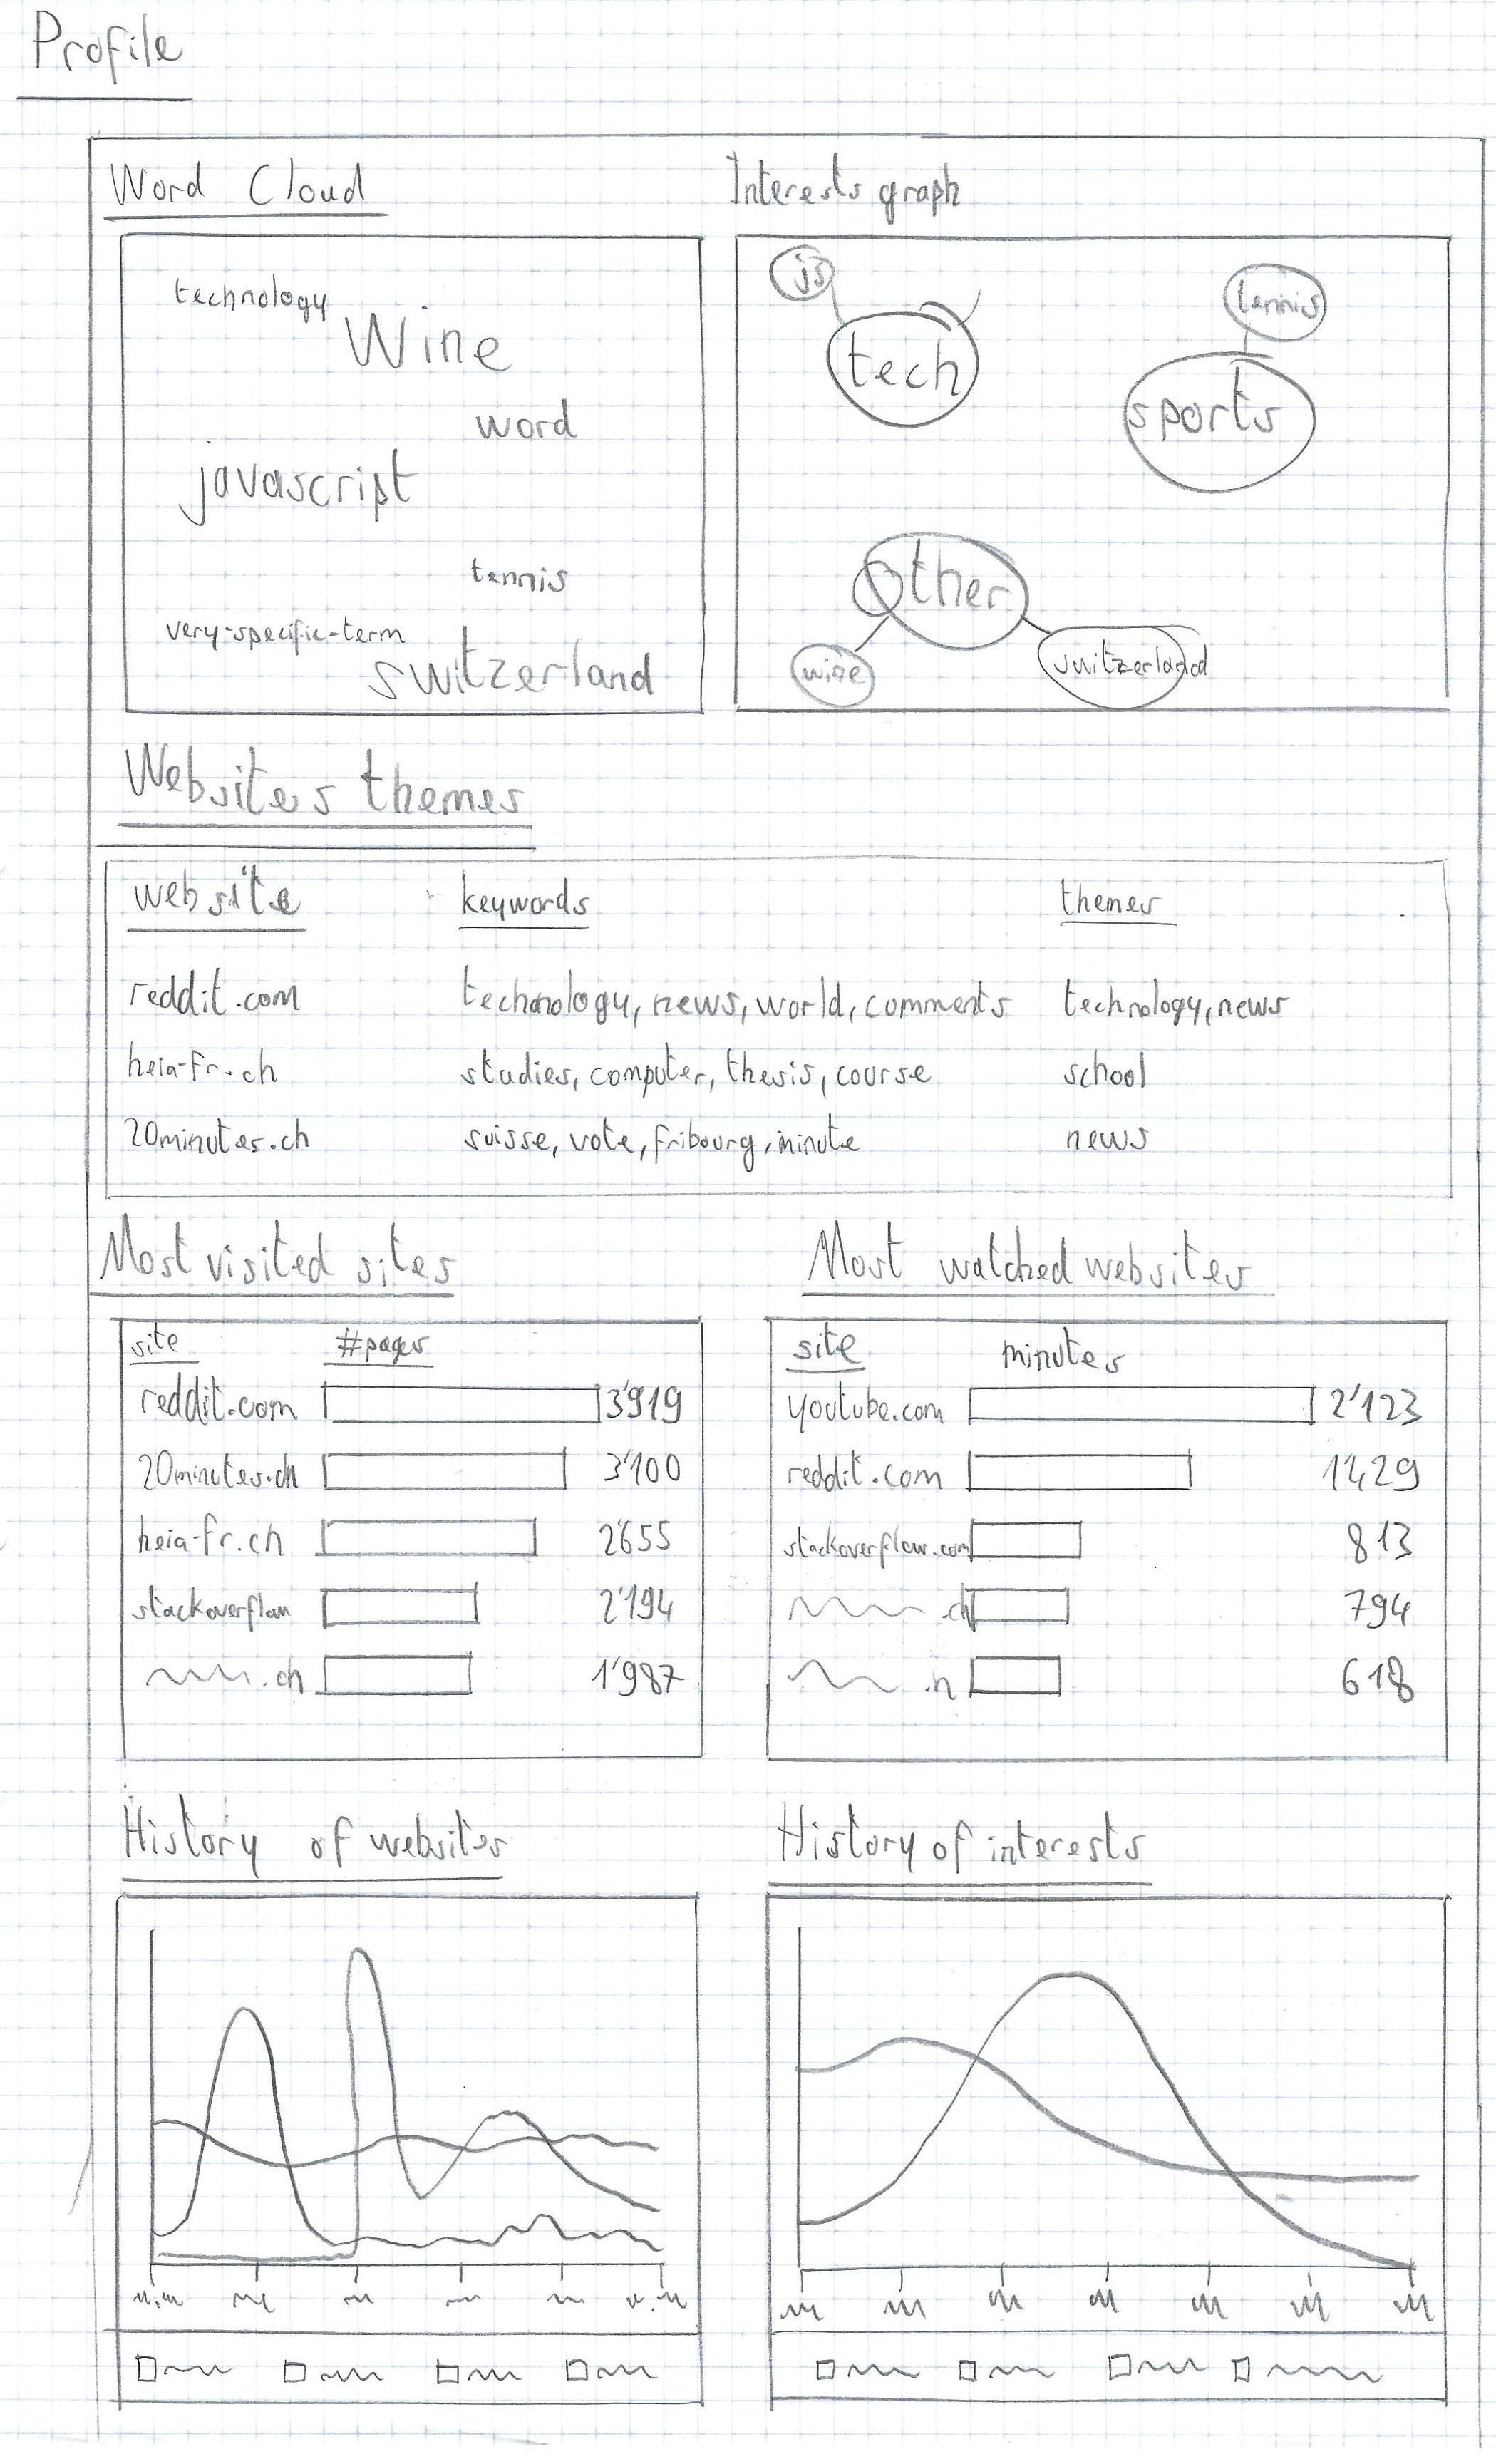
\includegraphics[width=0.8\textwidth]{images/design/mockup_profile}
			\caption{Maquette de la page de Profil}
			\label{d-mockup-profile}
		\end{figure}

		La page Profil cherche à montrer le résultat de l'analyse des pages visitées par l'utilisateur, tentant de retrouver et de lui montrer quels sont ses centres d'intérêts. 

		Voici les différentes concepts de visualisations montrées à l'utilisateur :

		\subsubsection{Wordcloud}

			Le wordcloud montre à l'utilisateur la liste des mots qu'il lit le plus fréquemment. Le visualisation est un amassage de mots de différentes tailles, placés d'une manière aléatoire sur un rectangle. Les mots les plus lus ont une taille plus grande afin d'attirer l'attention de l'utilisateur.

			Cette visualisation cherche à donner très rapidement une impression générale des thèmes que l'utilisateur parcourt lors de sa navigation.

		\subsubsection{Topics graph}

			Le "topics graph" cherche à rassembler les mots en thèmes, et monte d'une manière plus synthétique les thèmes estimés que l'utilisateur parcourt fréquamment. À chaque thème est lié un ou plusieurs mots, qui reprèsentent le thème d'une manière générale. Chaque cercle du graphe représente soit un thème, soit un mot.

			Le but de cette visualisation est de montrer que nous pouvons déduire des thèmes et ainsi montrer un traitement plus fin des intérêts de l'utilisateur, que simplement additionner une liste de mots. Dans le marketing, les thèmes découverts pourraient être utilisés pour labelliser les utilisateurs à qui faire apparaître une publicité.

	\subsection{Trackers}

		\begin{figure}[!h]
			\centering
			\includegraphics[width=0.8\textwidth]{images/design/mockup_trackers1}
			\caption{Maquette de la page de Trackers}
			\label{d-mockup-trackers1}
		\end{figure}

		\begin{figure}[!h]
			\centering
			\includegraphics[width=0.8\textwidth]{images/design/mockup_trackers2}
			\caption{Suite de la maquette de la page de Trackers}
			\label{d-mockup-trackers2}
		\end{figure}

\chapter{Implémentation}
%%%%%%%%%%%%%%%%%%%%%%%%%%
%                          %
% ----- INTRODUCTION ----- %
%                          %
%%%%%%%%%%%%%%%%%%%%%%%%%%


%
%
% WORDCLOUD
%
%

\section{Wordcloud}

	\subsection{Concept}

		Le wordcloud montre à l'utilisateur la liste des mots qu'il lit le plus fréquemment. Le visualisation est un amassage de mots de différentes tailles, placés d'une manière aléatoire sur un rectangle. Les mots les plus lus ont une taille plus grande afin d'attirer l'attention de l'utilisateur.

		Cette visualisation cherche à donner très rapidement une impression générale des thèmes que l'utilisateur parcourt lors de sa navigation.

		\begin{figure}[!h]
			\centering
			\subfloat[Maquette initiale de la vue]{\includegraphics[width=0.33\textwidth,valign=t]{images/design/pages/wordcloud_mockup}}
			\subfloat[Exemple de résultat final]{\includegraphics[width=0.66\textwidth,valign=t]{images/design/pages/wordcloud_final}}
			\caption{Maquette initiale et résultat final de la vue Wordcloud}
			\label{wordcloud_images}
		\end{figure}

		La figure~\ref{wordcloud_images} montre la différence entre la vue imaginée initialement et le résultat final.

	\subsection{Données}

		\subsubsection{Sources}

			Les données source servant à constituer cette visualisation sont :
			\begin{description}
				\item[Temps de visualisation] : Temps de visualisation total de chaque page. Ces données sont stockées dans la table \texttt{pagewatch} (figure \ref{table-content}).
				\item[Poids TF-IDF] : Poids final selon l'algorithme TF-IDF de chaque mot. Ces données sont stockées dans la table \texttt{computed\_tfidf} (figure \ref{table-computed-tfidf}).
			\end{description}
		\subsubsection{Algorithme}

			Afin de déterminer quels sont les mots affichés ainsi que leur taille sur la visualisation, on assigne un "poids" à chaque mot.

			La figure~\ref{wordcloud_algo} illustre le fonctionnement de l'algorithme utilisé :
			\begin{description}
				\item[A] On calcule le poids de chaque mot dans chaque document en effectuant la méthode de TF-IDF.

				\item[B] On effectue la somme du temps que l'utilisateur a passé à regarder chaque page visitée. Cette opération est effectuée sur le serveur, et l'interface obtient ce résultat en appelant l'endpoint \texttt{/api/mostWatchedSites} du serveur. Le résultat de cet appel est une liste de l'ensemble des pages web visitées, comprenant entre autres pour chaque page : 
				\begin{itemize}
					\item Son URL
					\item Le temps total de visite, en secondes
					\item Une liste des mots les plus significatifs selon TF-IDF ainsi que leur poids TF-IDF (normalisé entre 0 et 1)
				\end{itemize}
				
				On initialise un dictionnaire qui va contenir le poids de chaque mot.

				\item[C] Pour chaque page web, on multiplie l'indice TF-IDF de chaque mot avec le temps de visualisation de la page. On additionne ce résultat au poids actuel du mot.
				
				Une fois tous les mots de toutes les pages web traités, nous sommes en possession d'un dictionnaire nous indiquant le poids final de chaque mot. Ce poids est donc égal à la somme de l'indice TF-IDF du mot sur chaque page multiplié par le temps de visite sur cette page.
				
				\item[D] On trie les mots par leur poids final, et on ne conserve que les 200 premiers. Il s'agira des 200 mots présents sur le wordcloud.
				
				Pour chacun des 200 mots, leur taille sur le Wordcloud est égale à leur poids final.
			\end{description}

			\begin{figure}[!h]
				\centering
				\includegraphics[height=1\textwidth]{images/design/pages/wordcloud_algo}
				\caption{Algorithme utilisé pour le Wordcloud}
				\label{wordcloud_algo}
			\end{figure}

	\subsection{Implémentation}

		\subsubsection{Serveur}

			La somme du temps de visualisation des pages est calculée en direct par une commande MySQL, elle est donc constamment à jour.

			Le poids TF-IDF de chaque mot est stocké dans la base de données, mais n'est pas constamment rafraîchi. L'opération de calcul des poids TF-IDF est une opération ponctuelle qui doit être lancée sur l'entièreté de la base de données par l'administrateur. Cette opération ne nécessite cependant pas de redémarrage du serveur.

			La concaténation de ces résultats (ainsi que certains autres qui ne sont pas utilisés par cette visualisation) est servie par l'endpoint \texttt{/api/mostWatchedSites} dans une liste en JSON.

		\subsubsection{Interface}

			La page va s'occuper d'agréger les résultats reçus du serveur. Ensuite, elle utilise les librairies \texttt{d3-cloud} ainsi que \texttt{d3} pour générer la visualisation du Wordcloud.

\clearpage

%
%
% TOPICS LIST
%
%

\section{Topics List}

	\subsection{Concept}

		Le "Topics List" cherche à rassembler les mots en thèmes, et montre d'une manière plus synthétique les thèmes estimés que l'utilisateur parcourt fréquamment. À chaque thème est lié un ou plusieurs mots, qui reprèsentent le thème d'une manière générale. Chaque cercle du graphe représente soit un thème, soit un mot.

		Le but de cette visualisation est de montrer que nous pouvons déduire des thèmes et ainsi montrer un traitement plus fin des intérêts de l'utilisateur, que simplement additionner une liste de mots. Dans le marketing, les thèmes découverts pourraient être utilisés pour labelliser les utilisateurs à qui faire apparaître une publicité.

		\begin{figure}[!h]
			\centering
			\subfloat[Maquette initiale de la vue]{\includegraphics[width=0.33\textwidth,valign=t]{images/design/pages/topics_mockup}}
			\subfloat[Exemple de résultat final]{\includegraphics[width=0.66\textwidth,valign=t]{images/design/pages/topics_final}}
			\caption{Maquette initiale et résultat final de la vue Wordcloud}
			\label{topics_images}
		\end{figure}

		La figure~\ref{topics_images} montre la différence entre la vue imaginée et le résultat final. On note ici que le principe même de la vue ainsi que son nom sont différents qu'initialement.

	\subsection{Données}

		\subsubsection{Sources}

			Les données source servant à constituer cette visualisation sont :
			\begin{description}
				\item[Temps de visualisation] : Temps de visualisation total de chaque page. Ces données sont stockées dans la table \texttt{pagewatch} (figure \ref{table-content}).
				\item[Topics LDA] : Liste des topics générés par le modèle LDA. Ces données sont stockées dans la table \texttt{lda\_topics} (figure \ref{table-lda-topics}).
				\item[Topics par page] : Liste pré-caluclée des topics trouvés pour chaque page. Ces données sont stockées dans la table \texttt{current\_url\_topics} (figure \ref{table-current-url-topics}).
				\item[Intérêts utilisateur] : Liste des intérêts renseignés par l'utilisateur. Ces données sont stockées dans la table \texttt{user\_interests} (figure \ref{table-user-interests}).
				\item[Correspondances topic-intrêt] : Liste des correspondances entre topic et intérêt renseignés par l'utilisateur. Ces données sont stockées dans la table \texttt{current\_user\_tags} (figure \ref{table-current-user-tags}).
			\end{description}

		\subsubsection{Algorithme}

			Afin de déterminer quels sont les topics affichés ainsi que leur intérêt estimé, on assigne un "score" à chaque topic pour l'utilisateur.

			L'algorithme suivant, illustré par la figure~\ref{topics_algo}, est appliqué aux données sources :
			\begin{description}
				\item[A] On entraîne un modèle LDA avec un nombre défini de topics (typiquement 100) sur le contenu de l'ensemble des pages web, une page web représentant un document.
				
				Une fois le modèle LDA entraîné, on lui demande la liste des 100 topics générés par leur représentation en 5 mots. Cette liste de topics est enregistrée dans la base de données.

				\item[B] Pour chaque page enregistrée, on demande au modèle LDA quels sont les 5 topics les plus probables avec leur score de probabilité. Ces informations sont également enregistrées dans la base de données. Jusqu'ici, toutes ces opérations sont donc déjà calculées et se font avant le lancement du serveur. Elles ne sont pas mises à jour en temps réel.
				
				\item[C] On effectue la somme du temps que l'utilisateur a passé à regarder chaque page visitée. Cette opération est effectuée sur le serveur, et l'interface obtient ce résultat en appelant l'endpoint \texttt{/api/mostWatchedSites} du serveur. Le résultat de cet appel est une liste de l'ensemble des pages web visitées, comprenant entre autres pour chaque page : 
				\begin{itemize}
					\item Son URL
					\item Le temps total de visite, en secondes
					\item Une liste des topics les plus significatifs selon le modèle LDA ainsi que leur probabilité
				\end{itemize}

				\item[D] L'endpoint \texttt{/api/allTopics} renvoie la liste des topics générés par LDA ainsi que leur numéro d'identifiant.

				\item[E] L'endpoint \texttt{/api/getCurrentTags} renvoie la liste des associations que l'utilisateur a crée pour le modèle LDA courant. Il s'agit d'une liste de couples topicId $\longleftrightarrow$ interestId.

				\item[F] L'endpoint \texttt{/api/interestsList} renvoie la liste des 101 intérêts globaux à tous les utilisateurs.

				\item[G] On initialise un dictionnaire qui va contenir le score de chaque topic.
				
				Pour chaque page web, on multiplie la probabilité de chaque topic LDA avec le temps de visualisation de la page. On additionne ce résultat au score actuel du topic.
				
				Une fois tous les topics de toutes les pages web traités, nous sommes en possession d'un dictionnaire nous indiquant le score final de chaque topics. Ce score est donc égal à la somme de la probabilité du topic sur chaque page multiplié par le temps de visite sur cette page.
				
				\item[H] On trie les topics par leur score final, et on ne conserve que les 20 premiers. Il s'agira des 20 topics présents sur la page.

				\item[I] On sélectionne les centres d'intérêt de l'utilisateur, ainsi que les associations qu'il a déjà crée pour le modèle LDA actuel. On ajoute les associations aux topics de l'interface.
			\end{description}

			\begin{figure}[!h]
				\centering
				\includegraphics[height=1.35\textwidth]{images/design/pages/topics_algo}
				\caption{Algorithme utilisé pour le Topics List}
				\label{topics_algo}
			\end{figure}

	\subsection{Implémentation}

		\subsubsection{Serveur}

			La somme du temps de visualisation des pages est calculée en direct par une commande MySQL, elle est donc constamment à jour.

			Le modèle LDA est enregistré sur le disque local, et les résultats pré-calculés sont stocké dans la base de données, tout ceci n'est donc pas constamment rafraîchi. L'opération d'entraînement du modèle LDA est une opération ponctuelle qui doit être lancée sur l'entièreté de la base de données par l'administrateur. Cette opération nécessite le redémarrage du serveur, car de nombreuses mesures temporaires sont touchées.

			La concaténation de ces résultats (ainsi que certains autres qui ne sont pas utilisés par cette visualisation) est servie par l'endpoint \texttt{/api/mostWatchedSites} dans une liste en JSON. L'endpoint \texttt{/api/interestsList} est utilisé pour afficher le nom des centres d'intérêts, et l'endpoint \texttt{/api/getCurrentTags} donne l'ensemble des associations que l'utilisateur a crée entre ses centres d'intérêts, et les topics LDA actuels.

		\subsubsection{Interface}

			La page va s'occuper d'agréger les résultats reçus du serveur. La liste est ensuite générée sous forme d'un tableau HTML en passant par un composant Vue personnalisé. Les barres d'intérêt sont des éléments \texttt{progressbar} venant de Bootstrap.

\clearpage

%
%
% MOST WATCHED
%
%

\section{Most Watched}

	\subsection{Concept}

		Les pages "Most Watched" et "Most Visited" montrent deux informations, mais sous une forme semblable. Ces pages affichent quelles pages web et les domaines que l'utilisateur a visité le plus. Plus précisément, "Most Watched" s'intéresse au temps réel passé à lire chaque page, et "Most Visited" s'intéresse au nombre d'ouvertures de l'URL.

		Le but est ici de faire prendre conscience à l'utilisateur qu'il est possible de se rendre compte de son activité une page web, et un grand nombre d'ouvertures d'un lien ne veut pas forcément dire un grand intérêt pour cette page.

		On profite également de cet espace pour afficher les mots relatifs aux pages web qui ont le plus d'intérêt, afin de montrer qu'il est possible de déterminer quels sont les mots importants d'une page web simplement en la comparant au contenu des autres pages.

		La figure~\ref{mostwatched_images} montre la différence entre la vue imaginée et le résultat final.

		\begin{figure}[!h]
			\centering
			\subfloat[Maquette initiale de la vue]{\includegraphics[width=0.33\textwidth,valign=t]{images/design/pages/mostwatched_mockup}}
			\subfloat[Exemple de résultat final]{\includegraphics[width=0.66\textwidth,valign=t]{images/design/pages/mostwatched_final}}
			\caption{Maquette initiale et résultat final de la vue Most Watched}
			\label{mostwatched_images}
		\end{figure}

		Comme certaines pages web demandent une connexion pour être visualisées, par exemple la page d'accueil de \url{https://www.facebook.com}, nous omettons volontairement une liste de pages web dans ce classement, car nous n'avons pas d'informations intéressante sur leur contenu à montrer. En effet, nous ne téléchargeons volontairement pas de copie de la page vue par l'utilisateur pour des questions de protection de données privées. Notre serveur télécharge la version publique de l'URL visitée par l'utilisateur pour en déterminer son contenu. Ainsi, il ne fait pas sens d'analyser le contenu des pages générées dynamiquement par l'utilisateur.

	\subsection{Données}

		\subsubsection{Sources}

			Les données source servant à constituer cette visualisation sont :
			\begin{description}
				\item[Temps de visualisation] : Temps de visualisation total de chaque page. Ces données sont stockées dans la table \texttt{pagewatch} (figure \ref{table-content}).
				\item[Nombre de visites] : Nombre total d'ouvertures de chaque URL. Ces données sont stockées dans la table \texttt{pageviews} (figure \ref{table-pageviews}).
				\item[Poids TF-IDF] : Poids final selon l'algorithme TF-IDF de chaque mot. Ces données sont stockées dans la table \texttt{computed\_tfidf} (figure \ref{table-computed-tfidf}).
			\end{description}

		\subsubsection{Algorithme}

		Afin de déterminer quels sont les pages et les domaines affichés, on demande au serveur la liste triée des URLs les plus regardées et ouvertes.

			L'algorithme suivant, illustré par la figure~\ref{mostwatched_algo}, est appliqué aux données sources :
			\begin{description}
				\item[A] On calcule le poids de chaque mot dans chaque document en effectuant la méthode de TF-IDF.

				\item[B] On effectue la somme du temps que l'utilisateur a passé à regarder chaque page visitée. Cette opération est effectuée sur le serveur, et l'interface obtient ce résultat en appelant l'endpoint \texttt{/api/mostWatchedSites} du serveur. Le résultat de cet appel est une liste de l'ensemble des pages web regardées, comprenant entre autres pour chaque page : 
				\begin{itemize}
					\item Son URL
					\item Le temps total de visite, en secondes
					\item Une liste des mots les plus significatifs selon TF-IDF ainsi que leur poids TF-IDF (normalisé entre 0 et 1)
				\end{itemize}

				\item[C] On effectue la somme du nombre d'ouvertures de chaque page visitée. Cette opération est effectuée sur le serveur, et l'interface obtient ce résultat en appelant l'endpoint \texttt{/api/mostWatchedSites} du serveur. Le résultat de cet appel est une liste de l'ensemble des pages web visitées, comprenant entre autres pour chaque page : 
				\begin{itemize}
					\item Son URL
					\item Le nombre total d'ouvertures
					\item Une liste des mots les plus significatifs selon TF-IDF ainsi que leur poids TF-IDF (normalisé entre 0 et 1)
				\end{itemize}
				
				\item[D] Une fois la liste des pages les plus regardées obtenue, on ne conserve que les 10 premières d'entre-elles pour des raisons visuelles. Ces 10 premières pages sont alors affichées.

				\item[E] Ensuite, on cherche à agréger le temps de visualisation par domaine plutôt que par page, afin d'avoir une vue d'ensemble. On additionne donc le temps passé à regarder les pages d'un même domaine.

				\item[F] On trie la nouvelle liste de domaines crée par leur temps total de visualisation, et on ne garde également que les 10 premiers d'entre-eux pour les afficher.

				\item[G] On s'occupe ensuite du traitement du nombre d'ouvertures de chaque page. On ne conserve également que les 10 plus ouvertes d'entre-elles pour des raisons visuelles, elles sont alors affichées dans la liste.

				\item[H] Ensuite, on agrèger le nombre d'ouvertures par domaine plutôt que par page, afin d'avoir une vue d'ensemble. On additionne donc le temps passé à regarder les pages d'un même domaine.

				\item[I] On trie la nouvelle liste de domaines crée par leur temps total de visualisation, et on ne garde également que les 10 premiers d'entre-eux pour les afficher.
			\end{description}

			\begin{figure}[!h]
				\centering
				\includegraphics[height=0.8\textwidth]{images/design/pages/mostwatched_algo}
				\caption{Algorithme utilisé pour les pages "Most Watched" et "Most Visited"}
				\label{mostwatched_algo}
			\end{figure}

	\subsection{Implémentation}

		\subsubsection{Serveur}

			La somme du temps de visualisation des pages ainsi que du total d'ouvertues est calculée en direct par une commande MySQL, elle est donc constamment à jour.

			Le poids TF-IDF de chaque mot est stocké dans la base de données, mais n'est pas constamment rafraîchi. L'opération de calcul des poids TF-IDF est une opération ponctuelle qui doit être lancée sur l'entièreté de la base de données par l'administrateur. Cette opération ne nécessite cependant pas de redémarrage du serveur.

			La concaténation des résultats du temps total de visualisation ainsi que du nombre d'ouvertues est servi par respectivement l'endpoint \texttt{/api/mostWatchedSites}, et \texttt{/api/mostVisitedSites}.

		\subsubsection{Interface}

			La page va s'occuper d'agréger les résultats reçus du serveur. Chaque liste est ensuite générée sous forme d'un tableau HTML en passant par un composant Vue personnalisé. Les barres relatives à la quantité exprimée par chaque tableau ajoute un élément de comparaison visuel, et sont des éléments \texttt{progressbar} venant de Bootstrap.

\clearpage

%
%
% HISTORY
%
%

\section{History}

	\subsection{Concept}

		La page "History" permet de montrer à l'utilisateur la variation de ses habitudes au cours du temps durant lequel il a utilisé l'extension. Deux graphiques sont présents sur cette page : Le premier montre la tendence à visiter des pages relatées à certains topics, et l'autre montre la tendence dans la visite de pages contenant certains mots particuliers. Le but est ici de détecter d'éventuels intérêts passagers dans le temps.

		La figure~\ref{history_images} montre la différence entre la vue imaginée et le résultat final.

		\begin{figure}[!h]
			\centering
			\subfloat[Maquette initiale de la vue]{\includegraphics[width=0.3\textwidth,valign=t]{images/design/pages/history_mockup}}
			\subfloat[Exemple de résultat final]{\includegraphics[width=0.7\textwidth,valign=t]{images/design/pages/history_final}}
			\caption{Maquette initiale et résultat final de la vue History}
			\label{history_images}
		\end{figure}

	\subsection{Données}

		\subsubsection{Sources}

			Les données source servant à constituer cette visualisation sont :
			\begin{description}
				\item[Temps de visualisation] : Temps de visualisation total de chaque page. Ces données sont stockées dans la table \texttt{pagewatch} (figure \ref{table-content}).
				\item[Historique de visualisation] : Temps passé par jour sur chaque URL. Les données non agrégées proviennent de la table \texttt{pageviews} (figure \ref{table-pagewatch}).
				\item[Poids TF-IDF] : Poids final selon l'algorithme TF-IDF de chaque mot. Ces données sont stockées dans la table \texttt{computed\_tfidf} (figure \ref{table-computed-tfidf}).
				\item[Topics LDA] : Liste des topics générés par le modèle LDA. Ces données sont stockées dans la table \texttt{lda\_topics} (figure \ref{table-lda-topics}).
			\end{description}

		\subsubsection{Algorithme}

			Afin de déterminer quels sont les topics et les mots cumulant le plus d'intérêt, il est nécessaire de disposer de plusieurs sources de données et de les assembler afin d'arriver au résultat voulu. Ceci se fait en plusieurs étapes, distribuées entre le serveur et client.

			L'algorithme suivant, illustré par la figure~\ref{history_algo}, est appliqué aux données sources :
			\begin{description}
				\item[A] On calcule le poids de chaque mot dans chaque document en effectuant la méthode de TF-IDF.

				\item[B] On entraîne un modèle LDA avec un nombre défini de topics (typiquement 100) sur le contenu de l'ensemble des pages web, une page web représentant un document.
				
				Une fois le modèle LDA entraîné, on lui demande la liste des 100 topics générés par leur représentation en 5 mots. Cette liste de topics est enregistrée dans la base de données.

				\item[C] Pour chaque page enregistrée, on demande au modèle LDA quels sont les 5 topics les plus probables avec leur score de probabilité. Ces informations sont également enregistrées dans la base de données. Jusqu'ici, toutes ces opérations sont donc déjà calculées et se font avant le lancement du serveur. Elles ne sont pas mises à jour en temps réel.

				\item[D] On demande à la base de données de grouper le temps de visionnage (en secondes) en une somme par jour et par URL différente. Ceci se fait au travers d'une commande MySQL, et est calculé en temps réel.

				\item[E] Le résultat de l'étape précédente est disponible via l'endpoint\\
				\texttt{/api/historySites}.

				\item[F] On effectue la somme du temps que l'utilisateur a passé à regarder chaque page visitée. L'interface obtient ce résultat en appelant l'endpoint\\
				\texttt{/api/mostWatchedSites} du serveur. Le résultat de cet appel est une liste de l'ensemble des pages web regardées, comprenant entre autres une liste des mots les plus significatifs selon TF-IDF ainsi que leur poids TF-IDF (normalisé entre 0 et 1) pour chaque page.
				
				\item[G] L'endpoint \texttt{/api/allTopics} renvoie la liste des topics générés par LDA ainsi que leur numéro d'identifiant.

				\item[H] On cherche à savoir quels sont les mots où lesquels l'utilisateur a montré le plus d'intérêt afin de les afficher sur le graphe. Pour ceci, on multiplie la valeur TF-IDF de chaque mot par le temps passé à visualiser la page. La somme de ce calcul sur toutes les pages va nous donner l'"intérêt" final de l'utilisateur pour un mot particulier. On ne gardera ici que les 8 mots avec le plus grand intérêt estimé.

				\item[I] Finalement, pour chacun des 8 mots retenus, on affiche leur intérêt journalier sur le deuxième graphique, "Words history".

				\item[J] On cherche à savoir quels sont les topics où lesquels l'utilisateur a montré le plus d'intérêt afin de les afficher sur le graphe.

				Voici ce que l'on effectue sur chaque page : Pour chaque topic où sa valeur selon le modèle LDA sur cette page est au-dessus de 0.1, on estie que la page parle de ce topic et on compte le temps passé à visualiser la page dans la valeur de ce topic pour la journée.

				Finalement, on somme le temps passé sur chaque "topic". Le résultat de ce calcul sur toutes les pages va nous donner l'"intérêt" final de l'utilisateur pour un topic particulier. On ne gardera ici que les 8 topics avec le plus grand intérêt estimé.

				\item[K] Finalement, pour chacun des 8 topics retenus, on affiche leur intérêt journalier (qui est la même somme que précédamment, mais agrégée par jour au lieu de toute la période) sur le premier graphique, "Topics history".
			\end{description}

			\begin{figure}[!h]
				\centering
				\includegraphics[height=1.15\textwidth]{images/design/pages/history_algo}
				\caption{Algorithme utilisé pour les graphiques de la page "History"}
				\label{history_algo}
			\end{figure}

	\subsection{Implémentation}

		\subsubsection{Serveur}

			La somme du temps de visualisation effectuée en temps réel sur le serveur est faire par une commande MySQL qui s'occupe également d'"arrondir" chaque date de visualisation d'une page à la journée (au lieu de la seconde près, qui est la granularité utilisée dans la base de données).

		\subsubsection{Interface}

			Les données sont finalement transformées dans un format compatible et passées à une instance configurée de la librairie HighCharts, qui génère la visualisation du graphique sur la page.

\section{Trackers}

	\subsection{Concept}

		La vue "Trackers" comporte deux pages et 

	\subsection{Données}

		\subsubsection{Sources}

		\subsubsection{Algorithme}

	\subsection{Implémentation}

		\subsubsection{Serveur}

		\subsubsection{Interface}

\section{Stats}

	\subsection{Concept}

	\subsection{Données}

		\subsubsection{Sources}

		\subsubsection{Algorithme}

	\subsection{Implémentation}

		\subsubsection{Serveur}

		\subsubsection{Interface}

\section{Settings}

	\subsection{Concept}

	\subsection{Données}

		\subsubsection{Sources}

		\subsubsection{Algorithme}

	\subsection{Implémentation}

		\subsubsection{Serveur}

		\subsubsection{Interface}
\chapter{Résultats}
%%%%%%%%%%%%%%%%%%%%%%%%%%
%                          %
% ----- INTRODUCTION ----- %
%                          %
%%%%%%%%%%%%%%%%%%%%%%%%%%

\section{Validation}

	\subsection{Tests utilisateurs}

	Bla

\section{Résultats de la recherche}

	\subsection{Statistiques}

		\subsubsection{Profiling}

		\subsubsection{Trackers}

	\subsection{Implications}

\section{Conclusion}
\chapter{Conclusion}
\input{chapters/6_conclusion}

\begin{thebibliography}{9}

\bibitem{michal-kosinski}
  Michal Kosinski,
  \emph{Dr Michal Kosinski},
  \url{http://www.michalkosinski.com/},
  Consulté en ligne en Septembre 2017,
  2017.

\bibitem{mining-big-data}
  Michal Kosinski, Yilun Wang, Himabindu Lakkaraju and Jure Leskovec,
  \emph{Mining Big Data to Extract Patterns and Predict Real-Life Outcomes},
  \url{http://psycnet.apa.org/fulltext/2016-57141-003.pdf},
  Consulté en ligne en Octobre 2017,
  2017.

\bibitem{digital-footprints}
  Internet Society,
  \emph{Digital Footprints},
  \url{https://www.internetsociety.org/wp-content/uploads/2017/08/Digital20Footprints20-20An20Internet20Society20Reference20Framework.pdf},
  Consulté en ligne en Novembre 2017,
  Janvier 2014.

\bibitem{motherboard-data}
  Motherboard,
  \emph{The Data That Turned the World Upside Down},
  \url{https://motherboard.vice.com/en_us/article/mg9vvn/how-our-likes-helped-trump-win},
  Consulté en ligne en Octobre 2017,
  Janvier 2017.

\bibitem{kosinski-talk}
  Michal Kosinski,
  \emph{The End of Privacy, Keynote at CeBIT'17},
  \url{https://www.youtube.com/watch?v=DYhAM34Hhzc},
  Consulté en ligne en Octobre 2017,
  Mars 2017.

\bibitem{kaggle}
  Kaggle,
  \emph{Young People Survey},
  \url{https://www.kaggle.com/miroslavsabo/young-people-survey},
  Consulté en ligne en Octobre 2017,
  2013.

\bibitem{mypersonnality}
  Michal Kosinski,
  \emph{myPersonnality Project},
  \url{http://mypersonality.org},
  Consulté en ligne en Octobre 2017,
  2013.

\bibitem{analytics}
  Google,
  \emph{Google Solutions Analytics},
  \url{https://www.google.com/analytics},
  Consulté en ligne en Octobre 2017,
  2017.

\bibitem{analytics-usage}
  BuiltWith,
  \emph{Analytics Usage in Switzerland},
  \url{https://trends.builtwith.com/analytics/country/Switzerland},
  Consulté en ligne en Octobre 2017,
  2017.

\end{thebibliography}

\printglossary

\chapter*{Remerciements}
Je tiens à remercier ma superviseure Fatemi Nastaran pour m'avoir guidé lors des décisions à prendre, ainsi que Félicien Fleury pour m'avoir soutenu et guidé tout au long de ce projet.

\chapter*{Déclaration d'honneur}
Je, soussigné, Kewin Dousse, déclare sur l’honneur que le travail rendu est le fruit d’un travail personnel. Je certifie ne pas avoir eu recours au plagiat ou à toutes autres formes de fraudes. Toutes les sources d’information utilisées et les citations d’auteur ont été clairement mentionnées.

\bigskip
\bigskip

Lieu \hfil Date \hfil Signature

\appendix

\chapter{Historique des versions}
Voici l’historique des versions de ce document.

\begin{itemize}
	\item 0.1 : Template du document
	\item 0.2 : Rédaction de la partie Analyse
	\item 0.3 : Rédaction de la partie technique
	\item 1.0 : Rédaction de la plupart du reste du rapport
	\item 1.1 : Correction de la structure de chapitres dans les Prototypes
\end{itemize}

\chapter{Cahier des charges}
\section{Activités}

Le développement du projet peut se découper en plusieurs phases, qui elles-mêmes se divisent en plusieurs activités. Voici la liste de ces activités :

\begin{enumerate}
	\item Analyse
	\begin{enumerate}
		\item Item 1
		\item Item 2
	\end{enumerate}
	\item Conception
	\begin{enumerate}
		\item Item 1
		\item Item 2
	\end{enumerate}
	\item Implémentation
	\begin{enumerate}
		\item Item 1
		\item Item 2
	\end{enumerate}
	\item Résultats
	\begin{enumerate}
		\item Item 1
		\item Item 2
	\end{enumerate}
\end{enumerate}

\section{Planification}
Le projet comporte une série de dates-clé qu’il est important de respecter :
\begin{center}
   \begin{tabular}{ | l | c | r | }
     \hline
		Date & Semaine & Tâche \\ \hline
		\color{red}Lundi 18 septembre 2017 & Semaine P1 & Début du projet \\ \hline
		\color{red}Vendredi 9 février 2018 & Semaine P15 & Dépôt du rapport \\ \hline
		\color{red}26 février-9 mars 2017 & - & Défense orale \\ \hline
     \hline
   \end{tabular}
\end{center}

Les dates en rouge sont des dates de rendu officielles.
Les autres représentent des jalons dans l’avancement du projet.

\section{Diagramme de Gantt}
	\includegraphics[width=0.85\textwidth]{images/annexes/cdc/gantt}

\chapter{Documentation}
\section{Localisation}

	L’ensemble des documents du projet est disponible à l’adresse suivante :
	\url{https://forge.tic.heia-fr.ch/projects/vismed}

	Le code à son état du 15.07.2016 se trouve sur le dépôt git à l’adresse suivante :
	\url{https://gitlab.forge.hefr.ch/kewin.dousse/VisMed}

\section{Contenu}

	\subsection{Forge}

	Le projet présent sur la forge contient toutes les versions de chacun des documents suivants, sous l’onglet « Documents » :
	\begin{itemize}
		\item Les procès-verbaux réalisés durant le projet.
	\end{itemize}


% \chapter{Code source}
% \section{README.md}
\lstinputlisting[title=README.md]{appendix/src/README.md}

% \lstinputlisting[title=README.md,language=md]{appendix/src/README.md}


\chapter{Procès-verbaux}
Voici les documents des procès-verbaux réalisés.

\newpage

\includegraphics[width=1\textwidth]{images/annexes/pvs/DigFootprints_PV_15_09_2017}

\includegraphics[width=1\textwidth]{images/annexes/pvs/DigFootprints_PV_21_09_2017}

\includegraphics[width=1\textwidth]{images/annexes/pvs/DigFootprints_PV_28_09_2017}

\includegraphics[width=1\textwidth]{images/annexes/pvs/DigFootprints_PV_05_10_2017}

\includegraphics[width=1\textwidth]{images/annexes/pvs/DigFootprints_PV_10_10_2017}

\includegraphics[width=1\textwidth]{images/annexes/pvs/DigFootprints_PV_12_10_2017}

\includegraphics[width=1\textwidth]{images/annexes/pvs/DigFootprints_PV_16_10_2017}

\includegraphics[width=1\textwidth]{images/annexes/pvs/DigFootprints_PV_26_10_2017}

\includegraphics[width=1\textwidth]{images/annexes/pvs/DigFootprints_PV_01_11_2017}

\includegraphics[width=1\textwidth]{images/annexes/pvs/DigFootprints_PV_09_11_2017}

\includegraphics[width=1\textwidth]{images/annexes/pvs/DigFootprints_PV_13_11_2017}

\includegraphics[width=1\textwidth]{images/annexes/pvs/DigFootprints_PV_16_11_2017}

\includegraphics[width=1\textwidth]{images/annexes/pvs/DigFootprints_PV_23_11_2017}

\includegraphics[width=1\textwidth]{images/annexes/pvs/DigFootprints_PV_30_11_2017}

\includegraphics[width=1\textwidth]{images/annexes/pvs/DigFootprints_PV_05_12_2017}

\includegraphics[width=1\textwidth]{images/annexes/pvs/DigFootprints_PV_07_12_2017}

\includegraphics[width=1\textwidth]{images/annexes/pvs/DigFootprints_PV_12_12_2017}

\includegraphics[width=1\textwidth]{images/annexes/pvs/DigFootprints_PV_21_12_2017}

\includegraphics[width=1\textwidth]{images/annexes/pvs/DigFootprints_PV_09_01_2018}

\includegraphics[width=1\textwidth]{images/annexes/pvs/DigFootprints_PV_18_01_2018}

\end{document}

% https://www.sharelatex.com/blog/2013/08/02/thesis-series-pt1.htmlx